\begin{frame}[t, fragile]{Pandas Dataframes}
  \begin{block}{Definição}
    Estrutura de dados tabular muito similar a uma planilha..
  \end{block}
  \begin{columns}
    \begin{column}{0.5\textwidth}
        \begin{itemize}
          \item Estende a {\bf Serie} para multiplas dimensões
          \item Consiste de uma coleção ordenada de colunas
          \item Contém diversos valores com tipos diferentes
        \end{itemize}
    \end{column}

    \begin{column}{0.5\textwidth}
      \begin{center}
        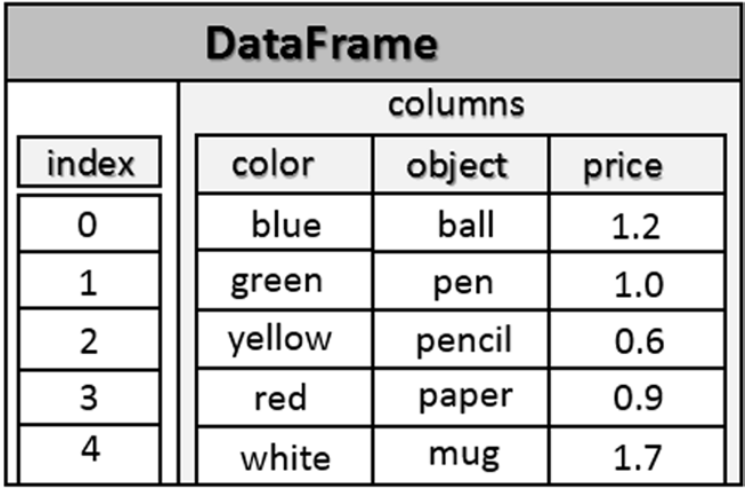
\includegraphics[scale=.21]{aula-2/figuras/pandas-dataframes-1.png}
      \end{center}
    \end{column}
  \end{columns}
\end{frame}
%
\begin{frame}[t, fragile, allowframebreaks]{Dataframe baseado em dicionário}
  \lstinputlisting[language=python]{aula-2/codigos/pandas/pandas-dataframes-1.py}  
\end{frame}
%
\begin{frame}[t, fragile, allowframebreaks]{Dataframe baseado em arquivo CSV}
  \lstinputlisting[language=python]{aula-2/codigos/pandas/pandas-dataframes-2.py}  
\end{frame}
%
\begin{frame}[t, fragile, allowframebreaks]{Acesso a valores de colunas}
  \lstinputlisting[language=python, firstline=5]{aula-2/codigos/pandas/pandas-dataframes-3.py}  
\end{frame}
%
\begin{frame}[t, fragile]{Acesso a valores de linhas}
  \lstinputlisting[language=python, firstline=6]{aula-2/codigos/pandas/pandas-dataframes-4.py}  
\end{frame}
%
\begin{frame}[t, fragile]{Operador $[ ]$}
  \begin{itemize}
    \item \verb![ ]!: tem funcionalidade limitada 
    \item Idealmente:
    \begin{itemize}
      \item para arrays bidimensionais
      \item \verb!um_array[linha, coluna]!
    \end{itemize}
    \item Em Pandas:
    \begin{itemize}
      \item \verb!loc!  (baseado em conteúdo)
      \item \verb!iloc! (baseado em posição)
    \end{itemize}
  \end{itemize}
\end{frame}
%
\begin{frame}[t, fragile]{Acesso a valores de linhas com {\bf loc}}
  \lstinputlisting[language=python, firstline=6]{aula-2/codigos/pandas/pandas-dataframes-5.py}  
\end{frame}
%
\begin{frame}[t, fragile]{Acesso a valores de linhas e colunas com {\bf loc}}
  \lstinputlisting[language=python, firstline=6]{aula-2/codigos/pandas/pandas-dataframes-6.py}  
\end{frame}
%
\begin{frame}[t, fragile]{Recapitulando}
  \begin{itemize}
    \item Colchetes \verb![ ]! 
    \begin{itemize}
      \item acesso a colunas: \verb!brics[["pais", "capital"]]!  
      \item acesso a linhas: somente via fatiamento \verb!brics[1:4]!
    \end{itemize}
    \item {\bf loc}
    \begin{itemize}
      \item acesso a linhas: \verb!brics.loc[["RU", "IN", "CH"]]!  
      \item acesso a colunas: \verb!brics.loc[:, ["pais", "capital"]]! 
      \item linhas e colunas: \verb!brics.loc[["RU", "IN", "CH"], ["pais", "capital"]]!    
    \end{itemize}
  \end{itemize}
\end{frame}
%
\begin{frame}[t, fragile]{Acesso a valores de linhas com {\bf iloc}}
  \lstinputlisting[language=python, firstline=6]{aula-2/codigos/pandas/pandas-dataframes-7.py}  
\end{frame}
%

\begin{frame}[t, fragile]{Acesso a valores de linhas e colunas com {\bf iloc}}
  \lstinputlisting[language=python, firstline=6]{aula-2/codigos/pandas/pandas-dataframes-8.py}  
\end{frame}
%


